\chapter{Background}
\label{sec:background}

In this section, we will introduce the theoretical elements necessary to complete the related work and the contributions illustrated in Chapters~\ref{sec:related} and~\ref{sec:contributions}. Our contributions range a wide span of physically based materials, including both scattering and non scattering media. We will describe both in this chapter (Sections~\ref{sec:scatteringtheory}~and~\ref{sec:brdftheory} respectively), with a brief introduction to basic radiometric concept (Section~\ref{sec:radiometry}). We will finally conclude (Section~\ref{sec:renderingparadigms}) with a more detailed description of the two main rendering paradigms we used to achieve our results, rasterization and ray tracing. A table with relevant notation used in this chapter is available at page~\pageref{sec:symbols}.

\section{Radiometry}
\label{sec:radiometry}
\begin{figure}
\centering
   \def\svgwidth{0.5\textwidth}
   \input{figures/radiance.pdf_tex} \\
\caption{Configuration to define radiance.} %The red rectangle shows where we estimated RMSE in Table \ref{table:quant}.}
\label{fig:radiance}
\end{figure}
Radiometry is a branch of physics that describes and measures electromagnetic radiation. In this section, we will define some basic radiometric quantities. In particular, we want to give a definition of radiance, the most useful quantity in describing light transport along rays.

First, let us consider an ideal point source of photons in space. This source emits a certain amount of energy $U$, measured in Joules $[J]$. The first quantity we derive is radiant flux or radiant power $\Phi$, defined as the amount of energy per second emitted by the light:
\begin{equation*}
\Phi = \frac{d U}{d t}  \siunit{\watt}.
\end{equation*}
The total flux represents the power the light emits in all directions. We usually want to be more descriptive on how a light or a surface is emitting light, since not all the sources we consider are ideal. First, we are interested on how light emission changes across directions.  We  define as \emph{radiant intensity} $I$ the amount of flux the light emits towards a specific direction $\vec{\omega}$:
\begin{equation*}
I(\vec{\omega}) = \frac{d \Phi}{d \omega}  \siunit{\watt \per \steradian},
\end{equation*}   
where $d \omega$ is an infinitesimal solid angle centered on direction $\vec{\omega}$. An isotropic point light, by definition, has constant intensity across all directions.

We now consider an infinitesimal surface area element $dA$ that receives light, with center point $\mathbf{x}$. We now define \emph{irradiance} as the amount of incoming flux received per unit area:
\begin{equation*}
E(\mathbf{x}) = \frac{d \Phi}{d A}  \siunit{\watt \per \square \metre}.
\end{equation*}
If the flux is emitted by the surface, we use the name \emph{radiosity} and define it with the symbol $B$.
The most simple irradiance is the one emitted by an isotropic point light. In this case, the irradiance at a distance $R$ from the point light is 
\begin{equation*}
E = \frac{\Phi}{4 \pi R^2} \siunit{\watt \per \square \metre}.
\end{equation*}
So, the farther we go from a point light, the less irradiance we receive, because the power $\Phi$ is spread across a larger area.

Finally, we combine the definitions of intensity and irradiance above into one, to define our last important basic radiometric quantity, \emph{radiance}:
\begin{equation*}
L(\mathbf{x}, \vec{\omega}) = \frac{d^2 \Phi}{dA \cos\theta d \omega}  \siunit{\watt \per \square \metre \per \steradian},
\end{equation*}
where $\cos \theta = \vec{n} \cdot \vec{\omega}$ is the cosine of the angle between the normal at $\mathbf{x}$ and the direction of evaluation. $dA \cos\theta$ is called the \emph{projected area element}. As irradiance, radiance can be incoming or outgoing from a specific point. We indicate these quantities with $L_i$ and $L_o$, respectively. In graphics, radiance is usually the most useful quantity for two main reasons. First, the other quantities can be easily computed from radiance through radiometric integrals:
\begin{figure}
\centering
   \def\svgwidth{0.8\textwidth}
   \input{figures/etendue.pdf_tex} \\
\caption{Configuration to prove the equality of radiance across a ray.} %The red rectangle shows where we estimated RMSE in Table \ref{table:quant}.}
\label{fig:etendue}
\end{figure}
\begin{equation*}
\begin{split}
\Phi &= \int_{\Omega^+} \int_{A} L(\mathbf{x}, \vec{\omega})  (\vec{n} \cdot \vec{\omega}) \ dA \ d {\omega}, \\
I(\vec{\omega}) &= \int_{A} L(\mathbf{x}, \vec{\omega})  (\vec{n} \cdot \vec{\omega}) \ dA,  \\
E(\mathbf{x}) &= \int_{\Omega^+} L(\mathbf{x}, \vec{\omega})  (\vec{n} \cdot \vec{\omega}) \ d {\omega}, 
\end{split}
\end{equation*}
where $\Omega^+$ and $A$ are the hemisphere around $\vec{n}$ and the total surface, respectively. Second, radiance carried by a ray \emph{in vacuo} is constant. We can prove this quite easily, with the aid of Figure~\ref{fig:etendue}. Note that for point $\mathbf{x}_o$, we have by definition $d \omega_o = \frac{d A_i \cos\theta_i}{r^2}$, and similarly  for $d \omega_i$. Then:
\begin{equation*}
\begin{split}
L_i(\mathbf{x}_i, \vec{\omega}_i) = \frac{d^2 \Phi}{d A_i \cos\theta_i d \omega_i} &= 
\frac{d^2 \Phi}{d A_i \cos\theta_i \frac{d A_o \cos\theta_o}{r^2}}  
\\ &= \frac{d^2 \Phi}{\frac{d A_i \cos\theta_i}{r^2} d A_o \cos\theta_o } 
= \frac{d^2 \Phi}{d A_o \cos\theta_o d \omega_o} = L_o(\mathbf{x}_o, \vec{\omega}_o).
\end{split}
\end{equation*}
Note that we assume that the flux does not vary across the path, which is generally true if no objects are in the way and there is no medium in between the two points causing scattering events. 

\section{Scattering Media}
\label{sec:scatteringtheory}
The first group of physically based materials we tackle is scattering media. We deal with efficient rendering of scattering media in Contributions~\ref{sec:juice} and~\ref{sec:interactivedirsss}, so we introduce relevant theory to better contextualize those contributions.

Scattering is the process photons go through once they hit an optically dense medium. Photons are deflected from their current path by electromagnetic forces, due to atom nuclei and atomic bonds. It is possible to model this process mathematically. We start by discussing one of such models, the radiative transfer equation, which is a local solution of the scattering process for a point in the medium. Then, we will provide a more global formulation of the scattering process as a function of light propagating between two surface points, the BSSRDF. We will then proceed to prove that the BSSRDF indeed respects the radiative transfer equation, and then describe two ways to render materials: one using the radiative transfer equation, one using BSSRDF. Finally, we will introduce three BSSRDF analytical models that can be used in rendering.

\subsection{The radiative transfer equation}
\label{sec:radiativetransfer}
\begin{figure}
\centering
\begin{tabular}{@{}c@{\hskip 1em}c@{}}
\def\svgwidth{0.45\textwidth}\input{figures/rte_absorption.pdf_tex} & 	 \def\svgwidth{0.45\textwidth}\input{figures/rte_emission.pdf_tex} \\
Absorption & Emission \\[1em]
\def\svgwidth{0.45\textwidth}\input{figures/rte_inscatter.pdf_tex} & 	 	 \def\svgwidth{0.45\textwidth}\input{figures/rte_outscatter.pdf_tex} \\
In-scattering &  Out-scattering \\
\end{tabular}
\caption{Individual processes in the local form of the radiative transfer equation: absorption, emission, in-scattering and out-scattering. The directional derivative $\vec{\omega} \cdot \nabla L(\mathbf{x}, \vec{\omega})$ corresponds on the variation over an infinitesimal length element $\text{d}r$ in direction $\vec{\omega}$. } 
\label{fig:rte_elements}
\end{figure}
The radiative transfer equation~\cite{Chandrasekhar1950} describes light propagation in scattering media. It is a particular form of the Boltzmann transport equation from thermodynamic system. In this section, we describe its integro-differential form, that describes how radiance $L(\mathbf{x}, \vec{\omega})$ varies at a point $\mathbf{x}$ in a scattering medium towards direction $\vec{\omega}$. For the sake of simplicity, from now on we assume a scattering media that respects linear optics (excluding i.e. fluorescent materials), and in the stationary state (i.e. the radiance $L$ is not changing in time). 

Traditionally, light traveling a medium is subject to four processes: absorption, emission, in-scattering and out-scattering. Each of these processes can be expressed in terms the directional derivative $\vec{\omega} \cdot \nabla L(\mathbf{x}, \vec{\omega})  \ \siunitnospace{\watt \per \cubic \metre \per \steradian}$. All effects are illustrated in Figure~\ref{fig:rte_elements}.

\textbf{Emission} increases the overall radiance of the ray by a term $q(\mathbf{x}, \vec{\omega})$:
\begin{equation*}
\vec{\omega} \cdot \nabla L(\mathbf{x}, \vec{\omega}) = q(\mathbf{x}, \vec{\omega}) \siunit{\watt \per \cubic \metre \per \steradian}.
\end{equation*} 
Emission describes how some form of energy (like heat) is becoming radiant energy.

\textbf{Absorption} is the dual effect of emission, where photons are absorbed by the material, and generally being transformed from radiant energy into heat energy. On the opposite hand of emission, the loss due to absorption is proportional to the radiance at the point $L$. The \emph{absorption coefficient} $\sigma_a(\mathbf{x}, \vec{\omega})  \siunitnospace{\per \metre} $ describes the amount of photons absorbed per unit traveled within the medium. In formulas,
\begin{equation*}
\vec{\omega} \cdot \nabla L(\mathbf{x}, \vec{\omega}) = - \sigma_a(\mathbf{x}, \vec{\omega}) L(\mathbf{x}, \vec{\omega}) \siunit{\watt \per \cubic \metre \per \steradian}.
 \end{equation*}
\textbf{Out-scattering} describes photons that are deflected from their original path $\vec{\omega}$  due to interaction with the atoms of the material. The effect is similar to absorption, with a different coefficient named \emph{scattering coefficient} $\sigma_s(\mathbf{x}, \vec{\omega}) \siunitnospace{\per \metre}$. This gives a loss of radiance that is similar to absorption:
\begin{equation*}
\vec{\omega} \cdot \nabla L(\mathbf{x}, \vec{\omega}) = - \sigma_s(\mathbf{x}, \vec{\omega}) L(\mathbf{x}, \vec{\omega})
 \siunit{\watt \per \cubic \metre \per \steradian}.
\end{equation*}
Absorption and out-scattering, given their similarities, are often combined into one effect, \emph{attenuation}, described by a value called the extinction coefficient $\sigma_t(\mathbf{x}, \vec{\omega}) =\sigma_s(\mathbf{x}, \vec{\omega}) + \sigma_a(\mathbf{x}, \vec{\omega}) \siunitnospace{\per \metre}$.

\textbf{In-scattering}, finally, describes the radiance aligning towards $\vec{\omega}$ from other scattering events. Let us consider another direction $\vec{\omega}'$ from $\mathbf{x}$. We define a probability distribution for a photon to scatter from $\vec{\omega}'$ towards an infinitesimal solid angle $d{\omega}$ around $\vec{\omega}$. This probability distribution is called the \emph{phase function}  $p(\mathbf{x}, \vec{\omega}', \vec{\omega}) \siunitnospace{ \per \steradian}$. With the phase function, and integrating over all directions, we get the effect of in-scattering.
\begin{equation*}
\vec{\omega} \cdot \nabla L(\mathbf{x}, \vec{\omega}) = \sigma_s(\mathbf{x}, \vec{\omega}) \int_{4\pi} L(\mathbf{x}, \vec{\omega}')  p(\mathbf{x}, \vec{\omega}', \vec{\omega}) d {\omega}'\siunit{\watt \per \cubic \metre \per \steradian}.
\end{equation*}
Note the multiplication by $\sigma_s$ to account for the right amount of scattering as we move along the ray. From the phase function, we can calculate the dimensionless radiometric property $g(\mathbf{x}, \vec{\omega})$, describing the mean cosine of the scattering angle between $\vec{\omega}$ and $\vec{\omega}'$ as
\begin{equation*}
g(\mathbf{x}, \vec{\omega}) = \int_{4\pi} (\vec{\omega}' \cdot \vec{\omega}) p(\mathbf{x}, \vec{\omega}', {\omega}) d{\omega}'
\siunit{-}.
\end{equation*}
As we will see, most analytical models describe a scattering medium in terms of the three coefficients $\sigma_s$, $\sigma_a$ and $g$, plus the ratio of the index of refraction inside the medium and the one outside the medium $\eta$.

We can now combine all terms to obtain the complete integro-differential form of the radiative transfer equation:
\begin{equation}
\label{eq:rte}
\vec{\omega} \cdot \nabla L(\mathbf{x}, \vec{\omega}) = q(\mathbf{x}, \vec{\omega}) - \sigma_t(\mathbf{x}, \vec{\omega}) L(\mathbf{x}, \vec{\omega}) + \sigma_s(\mathbf{x}, \vec{\omega}) \int_{4\pi} L(\mathbf{x}, \vec{\omega}')  p(\mathbf{x}, \vec{\omega}', \vec{\omega}) d {\omega}'.
\end{equation}
%
\subsection{The BSSRDF}
\label{sec:bssrdfgeneral}
\begin{figure}
\centering
   \def\svgwidth{0.8\textwidth}
   \input{figures/bssrdf_geometry.pdf_tex} \\
\caption{Configuration in which we define the BSSRDF for a generic surface.} %The red rectangle shows where we estimated RMSE in Table \ref{table:quant}.}
\label{fig:bssrdf_configuration}
\end{figure}
%
In Section~\ref{sec:radiometry}, we have defined radiometric quantities as either incoming or outgoing. We will now describe how radiometric quantities change between incoming and outgoing. This gives a way to describe light interaction due to a surface.

Let us first consider a surface $A$ illuminated by a light, as in Figure~\ref{fig:brdf_configuration}. Let us consider the element of flux $d\Phi_i$ arriving from direction $\vec{\omega}_i$ on a surface element $d A_i$ centered at a point $\mathbf{x}_i$. Due to surface interaction, part of the incoming light will emerge at a point $\mathbf{x}_o$, in direction $\vec{\omega}_o$. We consider the proportionality factor between the emitted radiance and the incoming flux:
\begin{equation}
\label{eq:bssrdf}
d L(\mathbf{x}_i, \vec{\omega}_i, \mathbf{x}_o, \vec{\omega}_o) = S(\mathbf{x}_i, \vec{\omega}_i, \mathbf{x}_o, \vec{\omega}_o) d \Phi_i(\mathbf{x}_i, \vec{\omega}_i)  \siunit{\watt \per \square \metre \per \steradian}.
\end{equation}
The factor $S$, dependent on the surface, is called \emph{bidirectional scattering-surface reflectance distribution function}, or BSSRDF for short~\cite{Nicodemus1977}. The units for the BSSRDF are $\siunitnospace{\per \square \metre \per \steradian}$. From the definition of BSSRDF and flux, we obtain right away the reflected radiance equation~\cite{Jensen2001}:
\begin{equation}
\label{eq:bssrdfintegral}
L(\mathbf{x}_o, \vec{\omega}_o) = \int_A \int_{\Omega^+} S(\mathbf{x}_i, \vec{\omega}_i, \mathbf{x}_o, \vec{\omega}_o) L_i(\mathbf{x}_i, \vec{\omega}_i) (\vec{n}_i \cdot \vec{\omega}_i) d A_i d {\omega}_i  \siunit{\watt \per \square \metre \per \steradian}.
\end{equation}
Note that we did not assume anything about the material, deriving the BSSRDF from purely radiometric quantities. The BSSRDF can be seen as a global formulation of scattering processes within the material.

Note that Equation~\ref{eq:bssrdfintegral} does not give the full outgoing radiance distribution $L_o$, since we need to add the radiance emitted by the body:
\begin{equation*}
L_o(\mathbf{x}, \vec{\omega}) = L_e(\mathbf{x}, \vec{\omega}) + L(\mathbf{x}, \vec{\omega}) .
\label{eq:renderingequation}
\end{equation*}
This equation gives the so called extended form of the rendering equation ~\cite{Jensen2001}. Given the physical nature of the BSSRDF, we can impose conservation of energy, so that the reflected light never increases:
\begin{equation}
\label{eq:bssrdfconservation}
0 \leq \int_A \int_\Omega S(\mathbf{x}_i, \vec{\omega}_i, \mathbf{x}_o, \vec{\omega}_o) (\vec{n}_i \cdot \vec{\omega}_i) d A_i d \vec{\omega}_i \leq 1 \siunit{-}.
\end{equation}
Moreover, the BSSRDF respects the Stokes-Helmholtz reciprocity principle~\cite{stokes_2009,Chandrasekhar1958}:
\begin{equation}
\label{eq:bssrdfreciprocity}
S(\mathbf{x}_i, \vec{\omega}_i, \mathbf{x}_o, \vec{\omega}_o) = 
S(\mathbf{x}_o, \vec{\omega}_o, \mathbf{x}_i, \vec{\omega}_i)  \siunit{\per \square \metre \per \steradian}.
\end{equation}

\subsection{Connecting BSSRDFs and the radiative transfer equation}

Given the above definition of BSSRDF (Equation~\ref{eq:bssrdf}), one may wonder how the BSSRDF is related to any scattering process at all, since it simply describes a relationship between an incoming and an outgoing radiometric quantity. In this section, starting from the definition of the BSSRDF, we will derive the local integro-differential form of the radiative transfer Equation~\ref{eq:rte}, to show how the BSSRDF fits nicely as a mathematical description of an underlying scattering process. Most of this derivation comes from Preisendorfer~\cite{Preisendorfer1965,Preisendorfer76}, where the BSSRDF is called \emph{scattering function}.

To show this relationship, we to define some mathematical operators. A operator in our context maps a function into another function, as does this  $\operator{Q}$ to integrate over an hemisphere:
\begin{equation*}
\operator{Q} = \int_\Omega [\ \ ] d\omega.
\end{equation*}
So, using the operator left associativity, $E = L\operator{Q}$ denotes the equation
\begin{equation*}
E(\mathbf{x}) = \int_\Omega L(\mathbf{x}, \vec{\omega}) d\omega.
\end{equation*}
Note that in this case operator $\operator{Q}$ maps the functional $L$ into functional $E$.
Where obvious, we drop the dependencies on $\mathbf{x}$ and $\omega$ from the operator for the sake of clarity. We can now define a new functional operator $\opa$, also called the \emph{standard operator}:
\begin{equation*}
\opa(a,b) = \int_a \int_{\Omega_i^+} [\ \ ] S(\mathbf{x}_i, \vec{\omega}_i, \mathbf{x}_o, \vec{\omega}_o) (\vec{n}_i \cdot \vec{\omega_i}) d \omega_i d A_i.
\end{equation*}
Where $S$ is the BSSRDF, $a$ and $b$ are parts of the surface of the medium containing $\mathbf{x}_i$ and $\mathbf{x}_o$, respectively, and $\Omega_i^+$ is the hemisphere oriented towards $\vec{n}_i$. This allows us to write $L = L_i \opa(a,b)$ for equation~\ref{eq:bssrdfintegral}, greatly simplifying notation.
%
\begin{figure}
\centering
   \def\svgwidth{0.8\textwidth}
   \input{figures/cylinder_geometry.pdf_tex} \\
\caption{Cylinder configuration to prove the radiance solution.} %The red rectangle shows where we estimated RMSE in Table \ref{table:quant}.}
\label{fig:cylinder}
\end{figure}
%
We want now to describe how radiance varies across a path. Let us consider the configuration of Figure~\ref{fig:cylinder}. In this figure, we have a path $P_r(\mathbf{x}_i,\vec{\omega})$ starting at $\mathbf{x}_i$, with direction $\vec{\omega}_o$ for $r$ units, terminating in $\mathbf{x}_o$ (so that $\mathbf{x}_o = \mathbf{x}_i + r \vec{\omega}_o$). Let us now consider a cylindrical medium $C$ with the same index of refraction as the surroundings, composed of three parts: a top circle $a$ on $\mathbf{x}_i$, a bottom circle $b$ on $\mathbf{x}_o$ and a flank surface $c$. We orient the cylinder so that the top $a$  points towards $-\vec{\omega}_o$, and the center of the cylinder is aligned with $P_r(\mathbf{x}_i,\vec{\omega}_o)$. This defines a direction for the hemispheres, e.g. $\Omega_i^+$ and $\Omega_i^-$ are the hemispheres centered in $\mathbf{x}_i$  and oriented towards or against $\vec{n}_i$, respectively. As a final bit of notation, we indicate with $L^+(a)$ some radiance $L(\mathbf{x}, \vec{\omega})$ where $\mathbf{x} \in a$ and $\vec{\omega} \in \Omega^+$.

At the steady state and by conservation of energy, the total radiance going out of the cylinder through the surface $b$ is:
\begin{equation}
\label{eq:steadystate}
L^-(b) = L^+(b)\opa(b,b) + L^-(a)\opa(a,b)  + L^-(c)\opa(c,b).
\end{equation}
We want now to find the behavior of the system at equilibrium, when the cylinder becomes thinner and thinner ($C\rightarrow P_r(\mathbf{x}_i,\vec{\omega}_o)$). We will analyze each one of the terms in Equation~\ref{eq:steadystate} independently. 

The first term on the right hand side of Equation~\ref{eq:steadystate} describes the part of $L^-(b)$ that stays inside due to reflection on $b$. This can be shown to tend to zero as the cylinder shrinks. This comes from the fact that for a transparent plane, all the radiance contribution passes through so none is reflected back. In formulas,
\begin{equation}
\label{eq:zerolimit}
\lim_{C\rightarrow P_r(\mathbf{x}_i,\vec{\omega}_o)} [L^+(b)\opa(b,b)] (\mathbf{x}_o, \vec{\omega}_o) = 0.
\end{equation}
The second term defines the radiance transmitted inbetween $a$ and $b$. As the cylinder shrink, the photons have less and less room to scatter within the cylinder, so only the photons staying directly on $\vec{\omega}$ (even if they scatter back and forth) will be considered at the end. Let us consider the limit:
\begin{equation*}
L_r^0(\mathbf{x}_o, \vec{\omega}_o) = \lim_{C\rightarrow P_r(\mathbf{x}_i,\vec{\omega}_o)} [L^-(a)\opa(a,b)] (\mathbf{x}_o, \vec{\omega}_o).
\end{equation*}
At the limit $a \rightarrow \mathbf{x}_i$, we have $L^-(a) = L^0(\mathbf{x}_i, \vec{\omega}_o)$, that can be brought out: 
\begin{equation}
\label{eq:l0r}
L_r^0(\mathbf{x}_o, \vec{\omega}_o) = L^0(\mathbf{x}_i, \vec{\omega}_o)\lim_{C\rightarrow P_r(\mathbf{x}_i,\vec{\omega}_o)} [\opa(a,b)] (\mathbf{x}_o, \vec{\omega}_o) = L^0(\mathbf{x}_i, \vec{\omega}_o) T_r(\mathbf{x}_i, \vec{\omega}_o),
\end{equation}
where the last term is called \emph{beam transmittance}, i.e. the amount of light blocked on the direct path. We define a dual term $1 -  T_r(\mathbf{x}_i, \vec{\omega})$, called \emph{beam attenuation}. The rate of change of beam attenuation per unit length at $\mathbf{x}_i$ on $\vec{\omega}$ is the extinction coefficient defined in Section~\ref{sec:radiativetransfer}:
\begin{equation*}
\sigma_t(\mathbf{x}_i, \vec{\omega}) = \lim_{r\rightarrow 0} \frac{1 - T_r(\mathbf{x}_i, \vec{\omega})}{r},
\end{equation*}
which leads to a natural definition for the beam transmittance
\begin{equation*}
T_r(\mathbf{x}_i, \vec{\omega}) = \exp\left(-\int_0^r \sigma_t(\mathbf{x}_i + r' \vec{\omega}, \vec{\omega}) dr'\right).
\end{equation*}
We now need to calculate the last term in the summation, which we call $L_r^*$:
\begin{equation*}
L_r^*(\mathbf{x}_o, \vec{\omega}_o) = \lim_{C\rightarrow P_r(\mathbf{x}_i,\vec{\omega}_o)} [L^-(c)\opa(c,b)] (\mathbf{x}_o, \vec{\omega}).
\end{equation*}
We will not include the full derivation, but by subdividing the cylinder into infinitesimally thin slices, each with its own transmittance, and then taking the limit, to obtain a integral form for $L_r^*$:
\begin{equation}
\label{eq:lastr}
L_r^*(\mathbf{x}_o, \vec{\omega}_o) = \int_0^r L_*(\mathbf{x}', \vec{\omega}_o) T_{r-r'}(\mathbf{x}', \vec{\omega}_o)  dr',
\end{equation}
where $\mathbf{x}' = \mathbf{x}_i + r' \vec{\omega}_o$ and where $L_*$ is the radiance per unit length
\begin{equation*}
L_*(\mathbf{x}', \vec{\omega}_o) = \lim_{r \rightarrow 0} \frac{L_r^*(\mathbf{x}_o, \vec{\omega}_o)}{r}.
\end{equation*}
By putting together \ref{eq:zerolimit}, \ref{eq:l0r} and \ref{eq:lastr} into \ref{eq:steadystate}, we obtain the following form:
\begin{equation}
\label{eq:fullformintegralpacked}
L_r(\mathbf{x}_o, \vec{\omega}_o) = L_r^0(\mathbf{x}_o, \vec{\omega}_o) + L_r^*(\mathbf{x}_o, \vec{\omega}_o),
\end{equation}
\begin{equation*}
L_r(\mathbf{x}, \vec{\omega}_o) =  L^0(\mathbf{x}_i, \vec{\omega}_o) T_r(\mathbf{x}_i, \vec{\omega}_o) + \int_0^r L_*(\mathbf{x}', \vec{\omega}_o) T_{r-r'}(\mathbf{x}', \vec{\omega}_o)  dr'.
\end{equation*}
We only need now to define $L_*$ in terms of $L$. For this derivation, let us still consider the configuration of Figure \ref{fig:sphere}, where we have a point $\mathbf{x}'$ and vector $\vec{\omega}'$ on the surface of a sphere $d$ surrounding a point $\mathbf{x}$ on path $P_r(\mathbf{x}_i,r)$ with direction $\vec{\omega} = \vec{\omega}_s$. It is possible to derive an approximation of $S$ for small $s$ as
\begin{equation*}
S(\mathbf{x}', \vec{\omega}', \mathbf{x}, \vec{\omega}) = \sigma_s(\mathbf{x}', \vec{\omega}', \vec{\omega}) \frac{s}{A_i'} + o(s).
\end{equation*}
$\mathbf{x}', \mathbf{x}$ are two points on the sphere, $s$ is the sphere radius, and $A_i'$ is the area of the sphere that would be lit by a light shined from direction $-\vec{\omega}'$. The term $\sigma_s(\mathbf{x}', \vec{\omega}', \vec{\omega}) = \sigma_s(\mathbf{x}', \vec{\omega}') p(\mathbf{x}', \vec{\omega}', \vec{\omega})$ is the non-normalized phase function. $o(s)$ is an error such as $\lim_{s\rightarrow 0} \frac{o(s)}{s} = 0$.
%
\begin{figure}
\centering
   \def\svgwidth{0.8\textwidth}
   \input{figures/sphere_geometry.pdf_tex} \\
\caption{Sphere configuration to prove the radiance solution.} %The red rectangle shows where we estimated RMSE in Table \ref{table:quant}.}
\label{fig:sphere}
\end{figure}
%
We can now recalculate $L_s^*$ {for the sphere configuration} using the approximation:
\begin{equation}
\begin{split}
L_s^*(\mathbf{x}, \vec{\omega}) &= \int_{A_i'} \int_{\Omega^-_i} L(\mathbf{x}', \vec{\omega}')  [\sigma_s(\mathbf{x}', \vec{\omega}', \vec{\omega}) \frac{s}{A_i'} + o(s)] (\vec{n}' \cdot \vec{\omega}') d\omega' dA_i'  \\
&= \int_{4\pi}  L(\mathbf{x}', \vec{\omega}')  [\sigma_s(\mathbf{x}', \vec{\omega}', \vec{\omega}) s + A_i' o(s)] (\vec{n}' \cdot \vec{\omega}') d\omega'\\
&= s \int_{4\pi}  L(\mathbf{x}', \vec{\omega}')  \sigma_s(\mathbf{x}', \vec{\omega}', \vec{\omega}) d\omega' + o(s) \int_{4\pi}  L(\mathbf{x}', \vec{\omega}') A_i'   d\omega'.
\end{split}
\end{equation}
As the sphere gets smaller $s\rightarrow 0$, the second term disappears with the $o(s)$, so that we finally obtain $L_*$ as
\begin{equation}
\label{eq:lstar}
L_*(\mathbf{x}, \vec{\omega}) = \lim_{s\rightarrow 0} \frac{L_s^*(\mathbf{x}, \vec{\omega})}{s} = \sigma_s(\mathbf{x}, \vec{\omega}) \int_{4\pi} L(\mathbf{x}, \vec{\omega}') p(\mathbf{x}, \vec{\omega}', \vec{\omega})   d\omega'.
\end{equation}
Putting it all together, we obtain the so called \emph{integral form} of the radiative transfer equation:
\begin{equation}
\begin{split}
\label{eq:integralformrte}
L_r(\mathbf{x}_o, \vec{\omega}_o) &=  L^0(\mathbf{x}_i, \vec{\omega}_o) T_r(\mathbf{x}_i, \vec{\omega}_o) + \\ &+\int_0^r \sigma_s(\mathbf{x}', \vec{\omega}_o) \int_{4\pi} L(\mathbf{x}', \vec{\omega}') p(\mathbf{x}', \vec{\omega}', \vec{\omega}_o)  d\omega' T_{r-r'}(\mathbf{x}', \vec{\omega}_o)  dr'.
\end{split}
\end{equation}
This form is described along a the extent of a path rather than a single point as in the integro differential form in Equation~\ref{eq:rte}. We now derive back that form by deriving the above across $r$, which is the same as a directional derivative $ \vec{\omega} \cdot \nabla$. Of the two terms on the right hand side of the equation above, the first becomes:
\begin{equation*}
\begin{split}
\frac{d}{dr} L^0(\mathbf{x}_i, \vec{\omega}_o) T_r(\mathbf{x}_i, \vec{\omega}_o) &= L^0(\mathbf{x}_i, \vec{\omega}_o) \frac{d}{dr}  T_r(\mathbf{x}_i, \vec{\omega}_o) \\
&= L^0(\mathbf{x}_i, \vec{\omega}_o) (-\sigma_t(\mathbf{x}_o, \vec{\omega}_o) T_r(\mathbf{x}_i, \vec{\omega}_o)) = -\sigma_t(\mathbf{x}_o, \vec{\omega}_o) L_r^0(\mathbf{x}_o, \vec{\omega}_o),
\end{split}
\end{equation*}
where the last step comes from Equation~\ref{eq:l0r}. As for the second term, we use the form from Equation~\ref{eq:lstar}:
\begin{equation*}
\begin{split}
\frac{d}{dr} L^*_r(\mathbf{x}_o, \vec{\omega}_o) &= \frac{d}{dr} \int_0^r L_*(\mathbf{x}', \vec{\omega}_o) T_{r-r'}(\mathbf{x}', \vec{\omega}_o)  dr' \\
&= \int_0^r L_*(\mathbf{x}', \vec{\omega}_o) \frac{d}{dr} T_{r-r'}(\mathbf{x}', \vec{\omega}_o)  dr' + L_*(\mathbf{x}_o, \vec{\omega}_o)
 \\
 &= -\sigma_t(\mathbf{x}, \vec{\omega}_o)  \int_0^r L_*(\mathbf{x}', \vec{\omega}_o) T_{r-r'}(\mathbf{x}', \vec{\omega}_o)  dr' + L_*(\mathbf{x}_o, \vec{\omega}_o) \\
 &= -\sigma_t(\mathbf{x}_o, \vec{\omega}_o) L^*_r(\mathbf{x}_o, \vec{\omega}_o) + L_*(\mathbf{x}_o, \vec{\omega}_o).
\end{split}
\end{equation*}
By putting it all together:
\begin{equation*}
\begin{split}
\frac{d}{dr} L_r(\mathbf{x}_o, \vec{\omega}_o) &= -\sigma_t(\mathbf{x}_o, \vec{\omega}_o) [L^0_r(\mathbf{x}, \vec{\omega}_o) + L^*_r(\mathbf{x}_o, \vec{\omega}_o)] + L_*(\mathbf{x}_o, \vec{\omega}_o) \\
&=  -\sigma_t(\mathbf{x}_o, \vec{\omega_o}) L_r(\mathbf{x}, \vec{\omega}_o) +  L_*(\mathbf{x}_o, \vec{\omega}_o) .
\end{split}
\end{equation*}
By dropping the dependency on $r$ and the $o$ subscript, and introducing the definition for $L_*$ (Equation~\ref{eq:lstar}) and the directional derivative symbol, we obtain the integro-differential form of the radiative  transfer equation
\begin{equation*}\vec{\omega} \cdot \nabla L(\mathbf{x}, \vec{\omega}) = - \sigma_t(\mathbf{x}, \vec{\omega}) L(\mathbf{x}, \vec{\omega}) + \sigma_s(\mathbf{x}, \vec{\omega}) \int_{4\pi} L(\mathbf{x}, \vec{\omega}')  p(\mathbf{x}, \vec{\omega}', \vec{\omega}) d \vec{\omega}'.
\end{equation*}
We can then add an additional term to account for emission, obtaining the form in Equation~\ref{eq:rte}.
\subsection{Global solution to the BSSRDF}
Now, we proved that the BSSRDF and the RTE are indeed connected through scattering theory. In this section, we will show an equivalent of the global solution~\ref{eq:bssrdfintegral} using the radiative transfer equation. To achieve this, we define the operator $\operator{S}^1$:
\begin{equation*}
\operator{S}^1 = \int_0^r \sigma_s(\mathbf{x}', \vec{\omega}) \int_{4\pi} [\ \ ] p(\mathbf{x}', \vec{\omega}', \vec{\omega})  (\vec{n} \cdot \vec{\omega}')  d\omega' T_{r-r'}(\mathbf{x}', \vec{\omega})  dr'.
\end{equation*}
Note on how this operator is similar to the second term of Equation~\ref{eq:integralformrte}. Now, let us consider a bounded medium, with a starting radiance distribution on the surface $L_0(\mathbf{x}_o, \vec{\omega})$ at a boundary point $\mathbf{x}_o$, where $\vec{\omega}_o$ points towards the inside of the medium. We can extend this initial radiance to any point $\mathbf{x} = \mathbf{x}_o + r \vec{\omega}$ of the medium:
\begin{equation*}
L^0(\mathbf{x}, \vec{\omega}) = L^0(\mathbf{x}_o, \vec{\omega}) T_r(\mathbf{x}_o, \vec{\omega}).
\end{equation*}
After defining $L^0$, we can define an $n$-ary radiance function $L^{n+1}$ recursively using operator $\operator{S}^1$:
\begin{equation*}
L^{n+1} = L^n \operator{S}^1.
\end{equation*}
The $n$-ary radiance can easily be calculated using a continuous application of the $S$ operator. If we define a new operator $\operator{S}^{n+1} = \operator{S}^1 \operator{S}^n$, one can show in a straightforward way that 
\begin{equation*}
L^n = L^0 \operator{S}^n
\end{equation*}
for every scattering order $n$.
We can bring this process to infinity by defining the two quantities:
\begin{equation*}
L = \sum_{j=0}^\infty L^j,\ \ \ \ \operator{S} = \sum_{j=0}^\infty \operator{S}^j.
\end{equation*}
In this particular case, we define $\operator{S}^0 = \operator{I}$, where $\operator{I}$, the identity operator, is a functional for which $f \operator{I} = f$ for every choice of $f$.
That leads to the formulation:
\begin{equation}
\label{eq:funcform}
L =  \sum_{j=0}^\infty L^j = \sum_{j=0}^\infty L^0 \operator{S}^j = L^0 \operator{S}.
\end{equation}
It is simple to prove that this formulation satisfies the integral form of the radiative transfer equation:
\begin{equation*}
\begin{split}
L &= L^0 \operator{S} \\
&= L^0 \left(\operator{I} + \operator{S}^1 + \sum_{j=2}^\infty \operator{S}^j \right) \\
&= L^0 \left( \operator{I} + \operator{S}^1 + \sum_{l=1}^\infty \operator{S}^{l+1} \right) \\
&= L^0 \left( \operator{I} + \left( \operator{I} + \sum_{l=1}^\infty \operator{S}^l \right) \operator{S}^1 \right)  \\
&= L^0 \left( \operator{I} + \operator{S} \operator{S}^1 \right)  \\
&= L^0 + (L^0 \operator{S}) \operator{S}^1   \\
L &= L^0 + L \operator{S}^1,   \\
\end{split}
\end{equation*}
where the last equation corresponds to the integral form of the radiative transfer equation in Equation~\ref{eq:integralformrte}.

Note that, since the solution of the radiance must be unique, the above calculated $L$ in functional form corresponds to the radiance $L$ calculated from Equation~\ref{eq:bssrdfintegral}. This tells us that the calculating the outgoing radiance through the BSSRDF is the same as integrating the radiance across all the possible paths within the material. This fundamental connections justifies comparing BSSRDF renderings, an approximation of equation~\ref{eq:bssrdfintegral}, with volume path tracing, in itself an approximation of Equation~\ref{eq:funcform}.

\subsection{Rendering scattering media}
\label{sec:renderingscattering}
Now, we want to use our formulas to derive a way to render scattering materials. The usual technique used in rendering to solve the rendering equation is Monte Carlo integration with importance sampling~\cite{Kalos2008}. Let us assume we need to solve the integral
\begin{equation*}
I = \int_a^b f(x) dx.
\end{equation*}
If we draw samples uniformly samples in $[a,b[$, we can define a $N$-th estimator for $I$:
\begin{equation*}
\hat{I}_N = \frac{b-a}{N} \sum_{i=1}^N f(x_i).
\end{equation*}
From the law of large numbers, $\hat{I}_N \rightarrow I$ for $N \rightarrow \infty$. To improve the convergence rate, we use importance sampling. If we know a distribution $\text{pdf}(x)$ that is somewhat close in shape to $f(x)$ and from which it is easy to draw samples $x_i \in [a,b]$. We can rewrite the integral $I$ as :
\begin{equation*}
I = \int_a^b \frac{f(x)}{\text{pdf}(x)} \text{pdf}(x) dx,
\end{equation*}
which we can evaluate again using Monte Carlo as:
\begin{equation*}
\hat{I}_N = \frac{b-a}{N} \sum_{i=1}^N \frac{f(x_i)}{\text{pdf}(x_i)}.
\end{equation*}
Where the $x_i$ follow the distribution $\text{pdf}(x)$. As before, $\hat{I}_N \rightarrow I$ for $N \rightarrow \infty$.

\subsubsection{Volume path tracing}
\label{sec:volumept}
Now let us apply importance sampling to obtain a first technique to render scattering materials, namely \emph{volume path tracing}~\cite{Rushmeier1988}. Volume path tracing is the classical formulation to render participating media, and it is usually used to generate reference images. In our Contribution~\ref{sec:juice}, where we strive for comparing images with photographs, we use a GPU-optimized version of volume path tracing to efficiently render glasses of apple juice.

We start by using the integral form of the radiative transfer equation~\ref{eq:integralformrte}. For the sake of this example, we assume a non emissive homogeneous medium, so that the coefficients do not depend on position and direction within the medium. We also assume index matched media, so we can simplify the interaction at the boundary. 

\begin{figure}
\centering
   \def\svgwidth{0.7\textwidth}
   \input{figures/vpt.pdf_tex} \\
\caption{Volumetric path tracing, with various paths going through the medium from camera $\mathbf{x}_c$ to light $\mathbf{x}_l$. Path (a) represents direct transmission to calculate $L^0(\mathbf{x}_t, \vec{\omega})$. Path (b) represents a path killed through absorption, while path (c) successfully exits the volume and connects to the light.} 
\label{fig:vpt}
\end{figure}

The algorithm, traces a ray from the camera direction $-\vec{\omega}$. The ray hits the surface at some point $\mathbf{x}_o$. We need to evaluate $L_r(\mathbf{x}_o, \vec{\omega})$. We first evaluate $r$ as the distance to the other side of the medium, hitting a point $\mathbf{x}_t = \mathbf{x}_o - r \vec{\omega}$. Because of the assumption of homogenous medium, the transmittance is easily evaluated:
\begin{equation*}
T_r(\mathbf{x}_t, \vec{\omega}) = \exp\left(-\int_0^r \sigma_t dr'\right) = e^{-\sigma_t r}.
\end{equation*}
We evaluate $L^0(\mathbf{x}_t, \vec{\omega})$ by continuing the path outside the medium in direction $-\vec{\omega}$. Now, we want to evaluate the second part of Equation~\ref{eq:integralformrte}, which is $L_r^*(\mathbf{x}_o, \vec{\omega})$ from Equation~\ref{eq:fullformintegralpacked}. For this, we use Monte Carlo integration with importance sampling. We first reparameterize the integral by imposing $s = r - r'$:
\begin{equation*}
L_r^*(\mathbf{x}_o, \vec{\omega}) = \int_0^r \sigma_s \int_{4\pi} L(\mathbf{x}', \vec{\omega}') p(\mathbf{x}', \vec{\omega}', \vec{\omega})  d\omega' T_{s}(\mathbf{x}', -\vec{\omega})  ds.
\end{equation*}
Note that $\mathbf{x}' = \mathbf{x}_o - s \vec{\omega} = \mathbf{x}_t + r' \vec{\omega}$. Now we can write the Monte Carlo estimator sampling both integrals at the same time:
\begin{equation}
\label{eq:lrintermediate}
\hat{L}_r^*(\mathbf{x}_o, \vec{\omega}) = \sum_{p=1}^N\sum_{q=1}^M \frac{\sigma_s L(\mathbf{x}_o - s_p, \vec{\omega}, \vec{\omega}'_q) p(\mathbf{x}_o - s_p, \vec{\omega}, \vec{\omega}'_q, \vec{\omega}) \exp(-\sigma_t s_p)}{\text{pdf}(s_p) \text{pdf}(\vec{\omega}'_q)}.
\end{equation}
For now, we assume that $s_p < r$, i.e. we are always sampling a point within the medium. Now, we need to choose the pdfs.  We can sample $s_p$ according to the formula:
\begin{equation*}
s_p = \frac{-\ln(1 - \xi)}{\sigma_t},
\end{equation*}
for $\xi \in [0,1)$, that corresponds to a $\text{pdf}(s_p) = \sigma_t \exp(-s_p \sigma_t)$. Once we have chosen $s_p$, we can move onto sampling $\vec{\omega}'_q$. For standard phase functions such as Henyey-Greenstein~\cite{Henyey1940}, it is possible to analytically find a way to importance sample a vector $\vec{\omega}'_q$. So, if the vector is carefully chosen, we have $\text{pdf}(\vec{\omega}'_p) = p(\mathbf{x}_o - s_p \vec{\omega}, \vec{\omega}'_q, \vec{\omega})$.

Plugging it in~\ref{eq:lrintermediate} we get the form
\begin{equation*}
\hat{L}_r^*(\mathbf{x}_o, \vec{\omega}) = \sum_{p=1}^N \sum_{q=1}^M \alpha L(\mathbf{x}_o - s_p, \vec{\omega}, \vec{\omega}'_q),
\end{equation*}
where $\alpha = \sigma_s / \sigma_t = \sigma_s / (\sigma_s + \sigma_a)  $ is called the \emph{single scattering albedo}. Note that $0 < \alpha < 1$.  Finally, we can introduce an additional importance sampling. We introduce a scattering probability $\text{pdf}_s = \alpha$. We decide then if we want to either scatter of absorb the photon, using russian roulette~\cite{Arvo1990}. If we decide to absorb the photon, we simply terminate the path. With this procedure in place , we get our final formulation
\begin{equation*}
\hat{L}_r^*(\mathbf{x}_o, \vec{\omega}) = \sum_{p=1}^N \sum_{q=1}^M\alpha \frac{L(\mathbf{x}_o - s_p, \vec{\omega}'_q)} {\text{pdf}_s} = \sum_{p=1}^N\sum_{q=1}^M L(\mathbf{x}_o - s_p, \vec{\omega}'_q). 
\end{equation*}
From this result, we see that we just need to recursively evaluate radiance to get the final result. At the next recursive step, we will evaluate a new $s_p$ and $\vec{\omega}'_q$, continue the process with probability $\alpha$ and so on. This creates a random walk within the medium, that does not terminate for $s_p < r$. If $s_p > r$, it means that we are exiting the medium. In this case, we continue path tracing from the exit point in the last evaluated direction $\vec{\omega}'_q$.

\subsubsection{The extended rendering equation}

Instead of using the various forms of the radiative transfer equation, we can use the form of the rendering equation in Equation~\ref{eq:bssrdfintegral}. Jensen and Buhler~\cite{Jensen2002} proposed one such technique, namely hierarchical integration. In general, we want to be able to sample points and directions on the surface of the scattering medium, so that we can solve the rendering equation via Monte Carlo integration using
\begin{equation*}
\hat{L}(\mathbf{x}_o, \vec{\omega}_o) \approx \sum_{p = 1}^N \sum_{q = 1}^M \frac{S(\mathbf{x}_{i,p}, \vec{\omega}_{i,q}, \mathbf{x}_o, \vec{\omega}_o) L_i(\mathbf{x}_{i,p}, \vec{\omega}_{i,q}) (\vec{n}_{i,p} \cdot \vec{\omega}_{i,q})}{\text{pdf}(\vec{\omega}_{i,q}) \text{pdf}(\mathbf{x}_{i,p})}.
\end{equation*}
We refer to our note in Appendix~\ref{sec:pointcloudnote} for a rendering technique that uses this estimator for the extended rendering equation, that we use in Contribution~\ref{sec:interactivedirsss} as an unbiased reference. Also, the technique from~\cite{Mertens2003} makes use of this approximation, which we derived again in Appendix~\ref{sec:mertensnote}.

\subsection{Analytical BSSRDF Models}
\label{sec:analyticalbssrdf}

So far, we have defined the BSSRDF as a proportionality constant between radiometric quantities. Given some assumptions about light propagation in materials, it is possible to derive analytical formulas for a BSSRDF for practical use in rendering. In the case of analytical models, Jensen et al.~\cite{Jensen2001} first provided an analyitical BSSRDF function based on the dipole solution in the work of Farrell et al.~\cite{Farrell1992} (the standard dipole). In this section, we outline the derivation of three analytical models, the standard dipole~\cite{Jensen2001}, the better dipole~\cite{dEon2012} and the directional dipole~\cite{Frisvad2014}. Our note in Appendix~\ref{sec:jensennote} provides additional derivation details for the interested reader. Note that more advanced dipoles exist, in particular the fully directional forward dipole~\cite{Frederickx2017}. We refer to the original paper for details on the derivation, which is out of the scope of this thesis.

Generically, the light exiting from a scattering medium at a point $\mathbf{x}_o$ at a direction $\vec{\omega}_o$ can be thought as coming from three contributions: direct transmission, single and multiple scattering. We define $\vec{\omega}_{21}$ as the refraction of $\vec{\omega}_o$ into the medium oriented towards the surface. Direct transmission is the contribution of the light coming from direction $-\vec{\omega}_{21}$ that does not scatter along the path (see Equation~\ref{eq:l0r}). The single scattering term comes from light that enters at any point of the medium, scatters once, then aligns with $\vec{\omega}_{21}$ to refract out in direction $\vec{\omega}_o$. The multiple scattering term is similar, but it includes light that has scattered more than once before exiting the medium. 

Single and multiple scattering are usually separated due to their different characteristics. Single scattering is highly peaked and directional, while multiple scattering can be handled as a stochastic process. The three analytical models we describe model the scattering of light as a diffusion process~\cite{Stam1995}. As such, the standard and better dipole model multiple scattering only, while the directional dipole models also part of the single scattering contribution. 

As before, we define operators to simplify notation:
\begin{equation*}
\operator{G} = \int_{4\pi} [\ \ ] d\omega, \ \ \ \vec{\operator{G}} = \int_{4\pi} [\ \ ] \vec{\omega} d\omega.
\end{equation*}
In radiative transport, we use spherical harmonics to simplify radiance~\cite{Eason1978}:
\begin{equation*}
L(\mathbf{x}, \vec{\omega}) = \frac{1}{4\pi}\phi(\mathbf{x}) + \frac{3}{4\pi} \vec{\omega} \cdot \mathbf{E}(\mathbf{x}),
\end{equation*}
where $\phi = L \operator{G}$ and $\mathbf{E} = L \vec{\operator{G}}$. Once we combine the radiative transfer equation and the diffusion approximation, we get the form:
\begin{equation}
\label{eq:telegraph}
(D \nabla^2 - \sigma_a)\phi(\mathbf{x}) = -Q_0(\mathbf{x}) + 3D \nabla \cdot \mathbf{Q}_1(\mathbf{x}, \vec{\omega}),
\end{equation}
where $Q_0 = q \operator{G}$ and $\mathbf{Q}_1 = q \vec{\operator{G}}$ are the integrals of the emission term in the radiative transfer equation $q(\mathbf{x}, \vec{\omega})$ (see Equation~\ref{eq:rte}). The choice of $q$, or \emph{source term} leads to different approximations. Standard and better dipole use a point source term, while the directional dipole uses a ray source. Equation~\ref{eq:telegraph} is a particular case of screened Poisson equation, that can be explicitly integrated~\cite{Fetter2003}. For a point source term, we obtain:
\begin{equation}
\label{eq:fluencepoint}
\phi(\mathbf{x}) = \frac{\alpha' \Phi_i}{4 \pi D} \frac{e^{-\sigma_\text{tr} r}}{r}.
\end{equation}
And for the ray source term, we get:
\begin{equation}
\label{eq:fluenceray}
\phi(\mathbf{x}) = \frac{\alpha' \Phi_i}{4 \pi D} \frac{e^{-\sigma_\text{tr} r}}{r} \left(1 + 3D \frac{1 + \sigma_\text{tr} r}{r} \cos\theta \right).
\end{equation}
Now that we have a formulation for the fluence, we need to connect it to the BSSRDF. First, we consider only the part of the BSSRDF depending on the diffusion approximation $S_d$. From the definition of BSSRDF in Equation~\ref{eq:bssrdf} and assuming a pure Fresnel boundary we get to this formulation in terms of the diffusive radiant exitance $M_d$
\begin{equation*}
S_d(\mathbf{x}_i, \vec{\omega}_i, \mathbf{x}_o)  =  \frac{1}{4\pi T_{12}C_\phi(1/\eta)} \frac{d M_d(\mathbf{x}_o)}{d \Phi_i(\mathbf{x}_i, \vec{\omega}_i)} .
\end{equation*} 
Through the diffusion approximation, we can approximate the diffusive radiant exitance $M_d$ as
\begin{equation*}
M_d(\mathbf{x}_o) =  C_\phi(\eta) \phi(\mathbf{x}_o) - C_\mathbf{E}(\eta) D \nabla\phi(\mathbf{x}_o) \cdot \vec{n}_o,
\end{equation*}
where $T_{12}$ is the incoming Fresnel coefficient, $C_\phi$ amnd $C_\mathbf{E}$ are the first two orders of Fresnel integrals, which can be approximated by analytical formulas~\cite{dEon2011}. The value $\eta$ is the index of refraction of the medium. By plugging in our solutions for the fluence in Equations~\ref{eq:fluencepoint} and~\ref{eq:fluenceray}, we get the analytical formula for a BSSRDF if we disregard the fact that light does not scatter outside the medium. In the case of a point source term, we obtain
\begin{equation*}
S_d(\mathbf{x}_i, \mathbf{x}_o)  = \frac{1}{4\pi C_\phi(1/\eta)} \frac{\alpha'}{4 \pi^2} \frac{e^{-\sigma_\text{tr} r}}{r^3} \left[ C_\phi(\eta) \frac{r^2}{D} + C_\mathbf{E}(\eta) (1 + \sigma_\text{tr} r) \mathbf{x} \cdot \vec{n}_o \right],
\end{equation*}
where $\mathbf{x} = \mathbf{x}_o - \mathbf{x}_i$ and $r = \|x\|$. This is the term used for the better dipole~\cite{dEon2012}. We can further simplify if we take the limit of the Fresnel integrals, obtaining $C_\phi(\eta) = 0$, $C_\mathbf{E}(\eta) = 1$ and $C_\phi(1/\eta) = 1/4$. This leads to
\begin{equation*}
S_d(\mathbf{x}_i, \mathbf{x}_o)  =  \frac{\alpha'}{4 \pi^2} \frac{e^{-\sigma_\text{tr} r}}{r^3} (1 + \sigma_\text{tr} r) \mathbf{x} \cdot \vec{n}_o,
\end{equation*}
which is used for standard dipole~\cite{Jensen2001}. Finally, if we use the ray source solution, we obtain
\begin{multline*}
S_d(\mathbf{x}_i, \vec{\omega}_i, \mathbf{x}_o)  = \frac{1}{4\pi C_\phi(1/\eta)} \frac{1}{4 \pi^2} \frac{e^{-\sigma_\text{tr} r}}{r^3} \bigg[ C_\phi(\eta) (\frac{r^2}{D} +  3 (1 + \sigma_\text{tr} r) \mathbf{x}\cdot\vec{\omega}_{12} ) \\ - C_\mathbf{E}(\eta) \left[3D (1 + \sigma_\text{tr} r) \vec{\omega}_{12} \cdot \vec{n}_o - \left((1 + \sigma_\text{tr} r) + 3D \frac{3 (1 + \sigma_\text{tr} r)  + (\sigma_\text{tr} r)^2}{r^2}\mathbf{x}\cdot\vec{\omega}_{12}\right) \mathbf{x} \cdot \vec{n}_o\right] \bigg],
\end{multline*}
which is used for he directional dipole~\cite{Frisvad2014}. 
%
\begin{figure}
\centering
\begin{tabular}{@{}c@{\hskip 1em}c@{}}
\def\svgwidth{0.5\textwidth}\input{figures/jensen_dipole.pdf_tex} &  \def\svgwidth{0.5\textwidth}\input{figures/dir_dipole.pdf_tex} \\
Standard and better dipole &  Directional dipole \\
\end{tabular}
\caption{Placement of virtual (red) and real (blue) sources for the dipoles described in the text.} 
\label{fig:bssrdfsources}
\end{figure}
%
As we mentioned, all these solutions are suitable only when light is allowed to scatter within an infinite medium with coefficients $\sigma_s$, $\sigma_a$ and $g$. To get a full BSSRDF, we need to introduce a boundary. We assume a refractive boundary with relative index of refraction $\eta$ as the ratio of the index of refraction of the incoming medium to the index of the refraction of the scattering medium. For the vast majority of analytical BSSRDFs, we derive a half-space solution based on a plane surface, then correct the formulas for non planar geometry.

To achieve a solution for a point $\mathbf{x}_o$ on a semi infinite plane with normal $\vec{n}_o$, we let the fluence $\phi$ vanish at the boundary. This leads for the following boundary condition for the diffusion approximation: 
\begin{equation*}
\phi(\mathbf{x}_o) - 2 A d_e (\vec{n}_o \cdot \nabla) \phi(\mathbf{x}_o) = 0
\end{equation*}
Where $d_e$ is called extrapolation distance, $A(\eta)$ is a term that accounts for mismatched index of refraction at the boundaries. The idea here is that the diffusion approximation matches better the exact solution if we let the fluence vanish not at the boundary, but at an \emph{extrapolated boundary} at distance $2 A d_e$ along the normal direction. This boundary condition can be satisfied by introducing two light sources, a positive \emph{real} source and a negative \emph{virtual} source, that together form a \emph{dipole configuration}.  Standard and better dipole use two point lights in the configuration to the left of Figure~\ref{fig:bssrdfsources}, with the real source (blue) below and the virtual source (red) above the surface. The directional dipole uses a real ray source on $\mathbf{x}_i$, and a virtual ray source above the surface (see right of Figure~\ref{fig:bssrdfsources}). The solutions for infinite media reported above are then evaluated for the real and the virtual source, and the results are then combined to obtain the final BSSRDF value for rendering. 

As we have seen, the complexity of the dipole greatly changes depending on how good the approximation is. The standard dipole, given its pure dependency on $r$, can be approximated quite efficiently, especially as a series of gaussian convolutions. The drawback of these dipole is that directional effects are lost, giving often an overly blurred result. In our contribution~\ref{sec:interactivedirsss} we will see how do we manage to create a interactive rendering technique that can handle the directional effects introduced by the directional dipole.

\section{Non-participating media}
\label{sec:brdftheory}
In this section, we will introduce some simplifications to the scattering theory introduced in Section~\ref{sec:scatteringtheory}. We introduce the description of the BRDF, a reflectance function far more widespread in real time application than the BSSRDF.   

\subsection{Transparent media}
\label{sec:glassdescr}
Multiple of our contributions make use of glass, in particular Contribution~\ref{sec:glass} and Contribution~\ref{sec:juice}. In this particular contribution, we describe glass as a non-scattering media, i.e. where $\sigma_s = 0$. This greatly simplifies the equations involved, leaving only the direct transmission term $L^0_r$ in Equation~\ref{eq:fullformintegralpacked}. This implies that the only noticeable effect is absorption, since $\sigma_t = \sigma_a$. Moreover, to define glass we need to define an interface, that in general is a specular interface defined by a relative index of refraction $\eta$. This is a good approximation for clear polished glass as the one we render in Contribution~\ref{sec:glass}. We discuss in contribution~\ref{sec:juice} how to include a diffuse term in the interface, since the glass in this case was scratched. We can easily render glass in a path tracing environment using the technique in in Section~\ref{sec:volumept}, leaving out the random walk and including the direct transmission contribution.

\subsection{Opaque media}
\subsubsection{The BRDF}
\label{sec:brdfsec}
\begin{figure}
\centering
   \def\svgwidth{0.9\textwidth}
   \input{figures/bsrdf_geometry.pdf_tex} \\
\caption{Configuration in which we define the BRDF for a generic surface.} %The red rectangle shows where we estimated RMSE in Table \ref{table:quant}.}
\label{fig:brdf_configuration}
\end{figure}

The methods that include scattering media we described in Section~\ref{sec:renderingscattering} are usually quite complex to render, requiring a high number of samples to converge. For many materials such as plastic or metal, the scattering process  is quite restricted around the point of emergence $\mathbf{x}_o$. For these particular materials, we can introduce some simplifications to obtain more tractable functions. We assume that the BSSRDF is limited across a small area around the emergence point $\mathbf{x}_o$, and zero everywhere else. In this configuration, we can assume that the radiance is constant across the plane ($L_i(\mathbf{x}_i, \vec{\omega}_i) \approx L_i(\vec{\omega}_i)$). We also need to assume that the material is locally isotropic, i.e. its properties do not change across the surface. In this case, we can approximate the outgoing radiance as:
\begin{equation*}
d L(\mathbf{x}_o, \vec{\omega}_o) \approx \int_A d L(\mathbf{x}_i, \vec{\omega}_i, \mathbf{x}_o, \vec{\omega}_o) = \int_A S(\mathbf{x}_i, \vec{\omega}_i, \mathbf{x}_o, \vec{\omega}_o) d \Phi_i(\mathbf{x}_i, \vec{\omega}_i).
\end{equation*}
By the definitions of flux and irradiance and the assumption of constant radiance outlined above, we obtain 
\begin{equation*}
\begin{split}
d L(\mathbf{x}_o, \vec{\omega}_o) &= \int_A S(\mathbf{x}_i, \vec{\omega}_i, \mathbf{x}_o, \vec{\omega}_o) L_i(\mathbf{x}_i, \vec{\omega}_i) (\vec{n} \cdot \vec{\omega}_i) d A_i d \omega_i  \\ &\approx L_i(\vec{\omega}_i) (\vec{n} \cdot \vec{\omega}_i) d \omega_i \int_A S(\mathbf{x}_i, \vec{\omega}_i, \mathbf{x}_o, \vec{\omega}_o)   d A_i \\ &= d E_i(\vec{\omega}_i) \int_A S(\mathbf{x}_i, \vec{\omega}_i, \mathbf{x}_o, \vec{\omega}_o) d A_i.
\end{split}
\end{equation*}
The last integral eliminates the dependency on $\mathbf{x}_i$, as it is a function purely dependent on the point of emergence $\mathbf{x}_o$ the two angular vectors $\vec{\omega}_i$ and $\vec{\omega}_o$. This proportionality constant between incoming irradiance and outgoing radiance $f_r$
\begin{equation}
\label{eq:brdf}
d L(\mathbf{x}_o, \vec{\omega}_o) = f_r(\mathbf{x}_o, \vec{\omega}_i, \vec{\omega}_o) d E_i(\mathbf{x}_o, \vec{\omega}_i),
\end{equation}
is called the \emph{bidirectional reflectance distribution function} (BRDF)~\cite{Nicodemus1977}. The BRDF is measured in $\siunitnospace{\per \steradian}$. As before, we can obtain the reflected radiance from the definition above:
\begin{equation}
\label{eq:brdfintegral}
L(\mathbf{x}, \vec{\omega}) = \int_\Omega f_r(\mathbf{x}, \vec{\omega}_i,  \vec{\omega}_o) L_i(\mathbf{x}, \vec{\omega}_i) (\vec{n} \cdot \vec{\omega}_i) d{\omega}_i  \siunit{\watt \per \square \metre \per \steradian}.
\end{equation}
This is called the reflected radiance equation. As before, we can add the emitted radiance $L_e$ to obtain the traditional form of the rendering equation~\cite{Kajiya1986}. We can easily extend the two properties of the BSSRDF in Equations~\ref{eq:bssrdfconservation} and~\ref{eq:bssrdfreciprocity}. Conservation of energy imposes
\begin{equation*}
0 \leq \int_\Omega f_r(\mathbf{x}, \vec{\omega}_i,  \vec{\omega}_o)  (\vec{n} \cdot \vec{\omega}_i) d{\omega}_i \leq 1.
\end{equation*}
On the other hand, Helmholtz reciprocity gives
\begin{equation*}
f_r(\mathbf{x}, \vec{\omega}_i,  \vec{\omega}_o) = f_r(\mathbf{x}, \vec{\omega}_o,  \vec{\omega}_i).
\end{equation*}
From the reflectance equation above, we can see why BRDFs are usually employed in real time applications, since BRDF require one less integral to solve (compare Equations~\ref{eq:brdfintegral} and~\ref{eq:bssrdfintegral}). We then use BRDFs in our Contributions~\ref{sec:glass},~\ref{sec:srt}~and~\ref{sec:vrbrdf} where the focus is not specific to scattering media. In applications such as games we may have a finite number of point and directional lights, which simplifies the integral in Equation~\ref{eq:brdfintegral} to a sum over all the lights.

\subsubsection{Empirical BRDFs}
\label{sec:empiricalbrdf}
\begin{figure}
\centering
\begin{tabular}{@{}c@{\hskip 1em}c@{}}
\def\svgwidth{0.45\textwidth}\input{figures/brdf_representation_simple.pdf_tex} &  \def\svgwidth{0.45\textwidth}\input{figures/brdf_representation_merl.pdf_tex} \\
Polar representation &  Rusinkiewicz representation \\
$f_r(\theta_i, \phi_i, \theta_o, \phi_o)$ &  $f_r(\theta_h, \phi_h, \theta_d, \phi_d)$ \\
\end{tabular}
\caption{Different representations for BRDFs. To the left, standard representation using polar coordinates. To the right, the representation from~\cite{Rusinkiewicz1998}. } 
\label{fig:brdfrepr}
\end{figure}

Given the low dimensionality of the BRDF, it is possible to actually measure and tabulate it, so that it can be used in future renderings. We use tabulated BRDFs multiple times in our Contributions~\ref{sec:glass} and~\ref{sec:vrbrdf}, given that they allows us to easily achieve a photorealistic look. If we assume a non-spatially varying BRDF (dropping the dependency from $\mathbf{x}_o$ in Equation~\ref{eq:brdf}) and expressing each vector $\vec{\omega}$ in terms of its polar angles $\theta, \phi$, we obtain a four dimensional function:
\begin{equation*}
f_r(\mathbf{x}, \vec{\omega}_i,  \vec{\omega}_o) = f_r(\theta_i, \phi_i, \theta_o, \phi_o).
\end{equation*}
Moreover, from now on we assume the BRDF to be \emph{isotropic}, so that it depends only on the relative angle $\phi_\text{diff} = \phi_o - \phi_i$:
\begin{equation*}
f_r^\text{iso}(\theta_i, \phi_i, \theta_o, \phi_o) = f_r^\text{iso}(\theta_i, \theta_o, \phi_\text{diff}).
\end{equation*}
Anisotropic materials (e.g. brushed metal) are rarer in nature and are usually created using some sort of manufacturing process.
This na\"ive representation, presented in Figure~\ref{fig:brdfrepr}, can be used to store BRDFs in a compact way, though with some issues. Generally, BRDFs tend to have a highly peaked region around the half vector:
\begin{equation*}\vec{\omega}_h = \frac{\vec{\omega}_i + \vec{\omega}_o}{\|\vec{\omega}_i + \vec{\omega}_o\|},
\end{equation*}
where there is usually a strong peak due to reflection, or \emph{specular highlight}. If we use the na\"ive parametrization, we would encounter some discretization issues around $\vec{\omega}_h$. To avoid this loss of precision, it is important to represent the BRDF more accurately around the half vector. So for measured datasets such as the MERL dataset~\cite{Matusik2003}, the Rusinkiewicz half-difference parameterization is used (see Figure~\ref{fig:brdfrepr}). This representation measures angles relative to the half vector instead of the surface normal:
\begin{equation*}
f_r(\mathbf{x}, \vec{\omega}_i,  \vec{\omega}_o) = f_r(\theta_h, \phi_h, \theta_d, \phi_d),
\end{equation*}
where $\theta_h, \phi_h$ are the spherical coordinates of $\vec{\omega}_h$, and where $\theta_d, \phi_d$ are the spherical coordinates of $\vec{\omega}_i$ rotated so that $\vec{\omega}_h$ matches the reference frame of $\vec{n}$. In this case,  isotropic materials can be described by dropping the dependency on $\phi_d$, i.e. the overall rotation of the system around the normal.

After we have chosen our representation, we can pack our isotropic BRDF in a 3D data structure. Note that similar packing representations exist also for BSSRDFs~\cite{Donner2009}, but the high dimensionality of the BSSRDF (5 up to 14 dimensions) renders these representations somewhat less practical. See the note in Appendix~\ref{sec:bssrdfnote} for a derivation on how to compute a simulated empirical BSSRDF. 

\section{Rendering techniques} 
\label{sec:renderingparadigms}

In the previous sections, we introduced theory and algorithms for rendering physically based materials, without going into details on how the different algorithms are implemented. To conclude our background section, we introduce two of the main paradigms used to render physically based materials on GPUs, namely rasterization and ray tracing. In our contribution, we use both techniques (rasterization in Contributions~\ref{sec:interactivedirsss}~and~\ref{sec:vrbrdf}, ray tracing in Contributions~\ref{sec:glass},~\ref{sec:juice} and~\ref{sec:srt}), choosing either one depending on the application constraints.

\subsection{Rasterization}

\begin{figure}
\centering
	 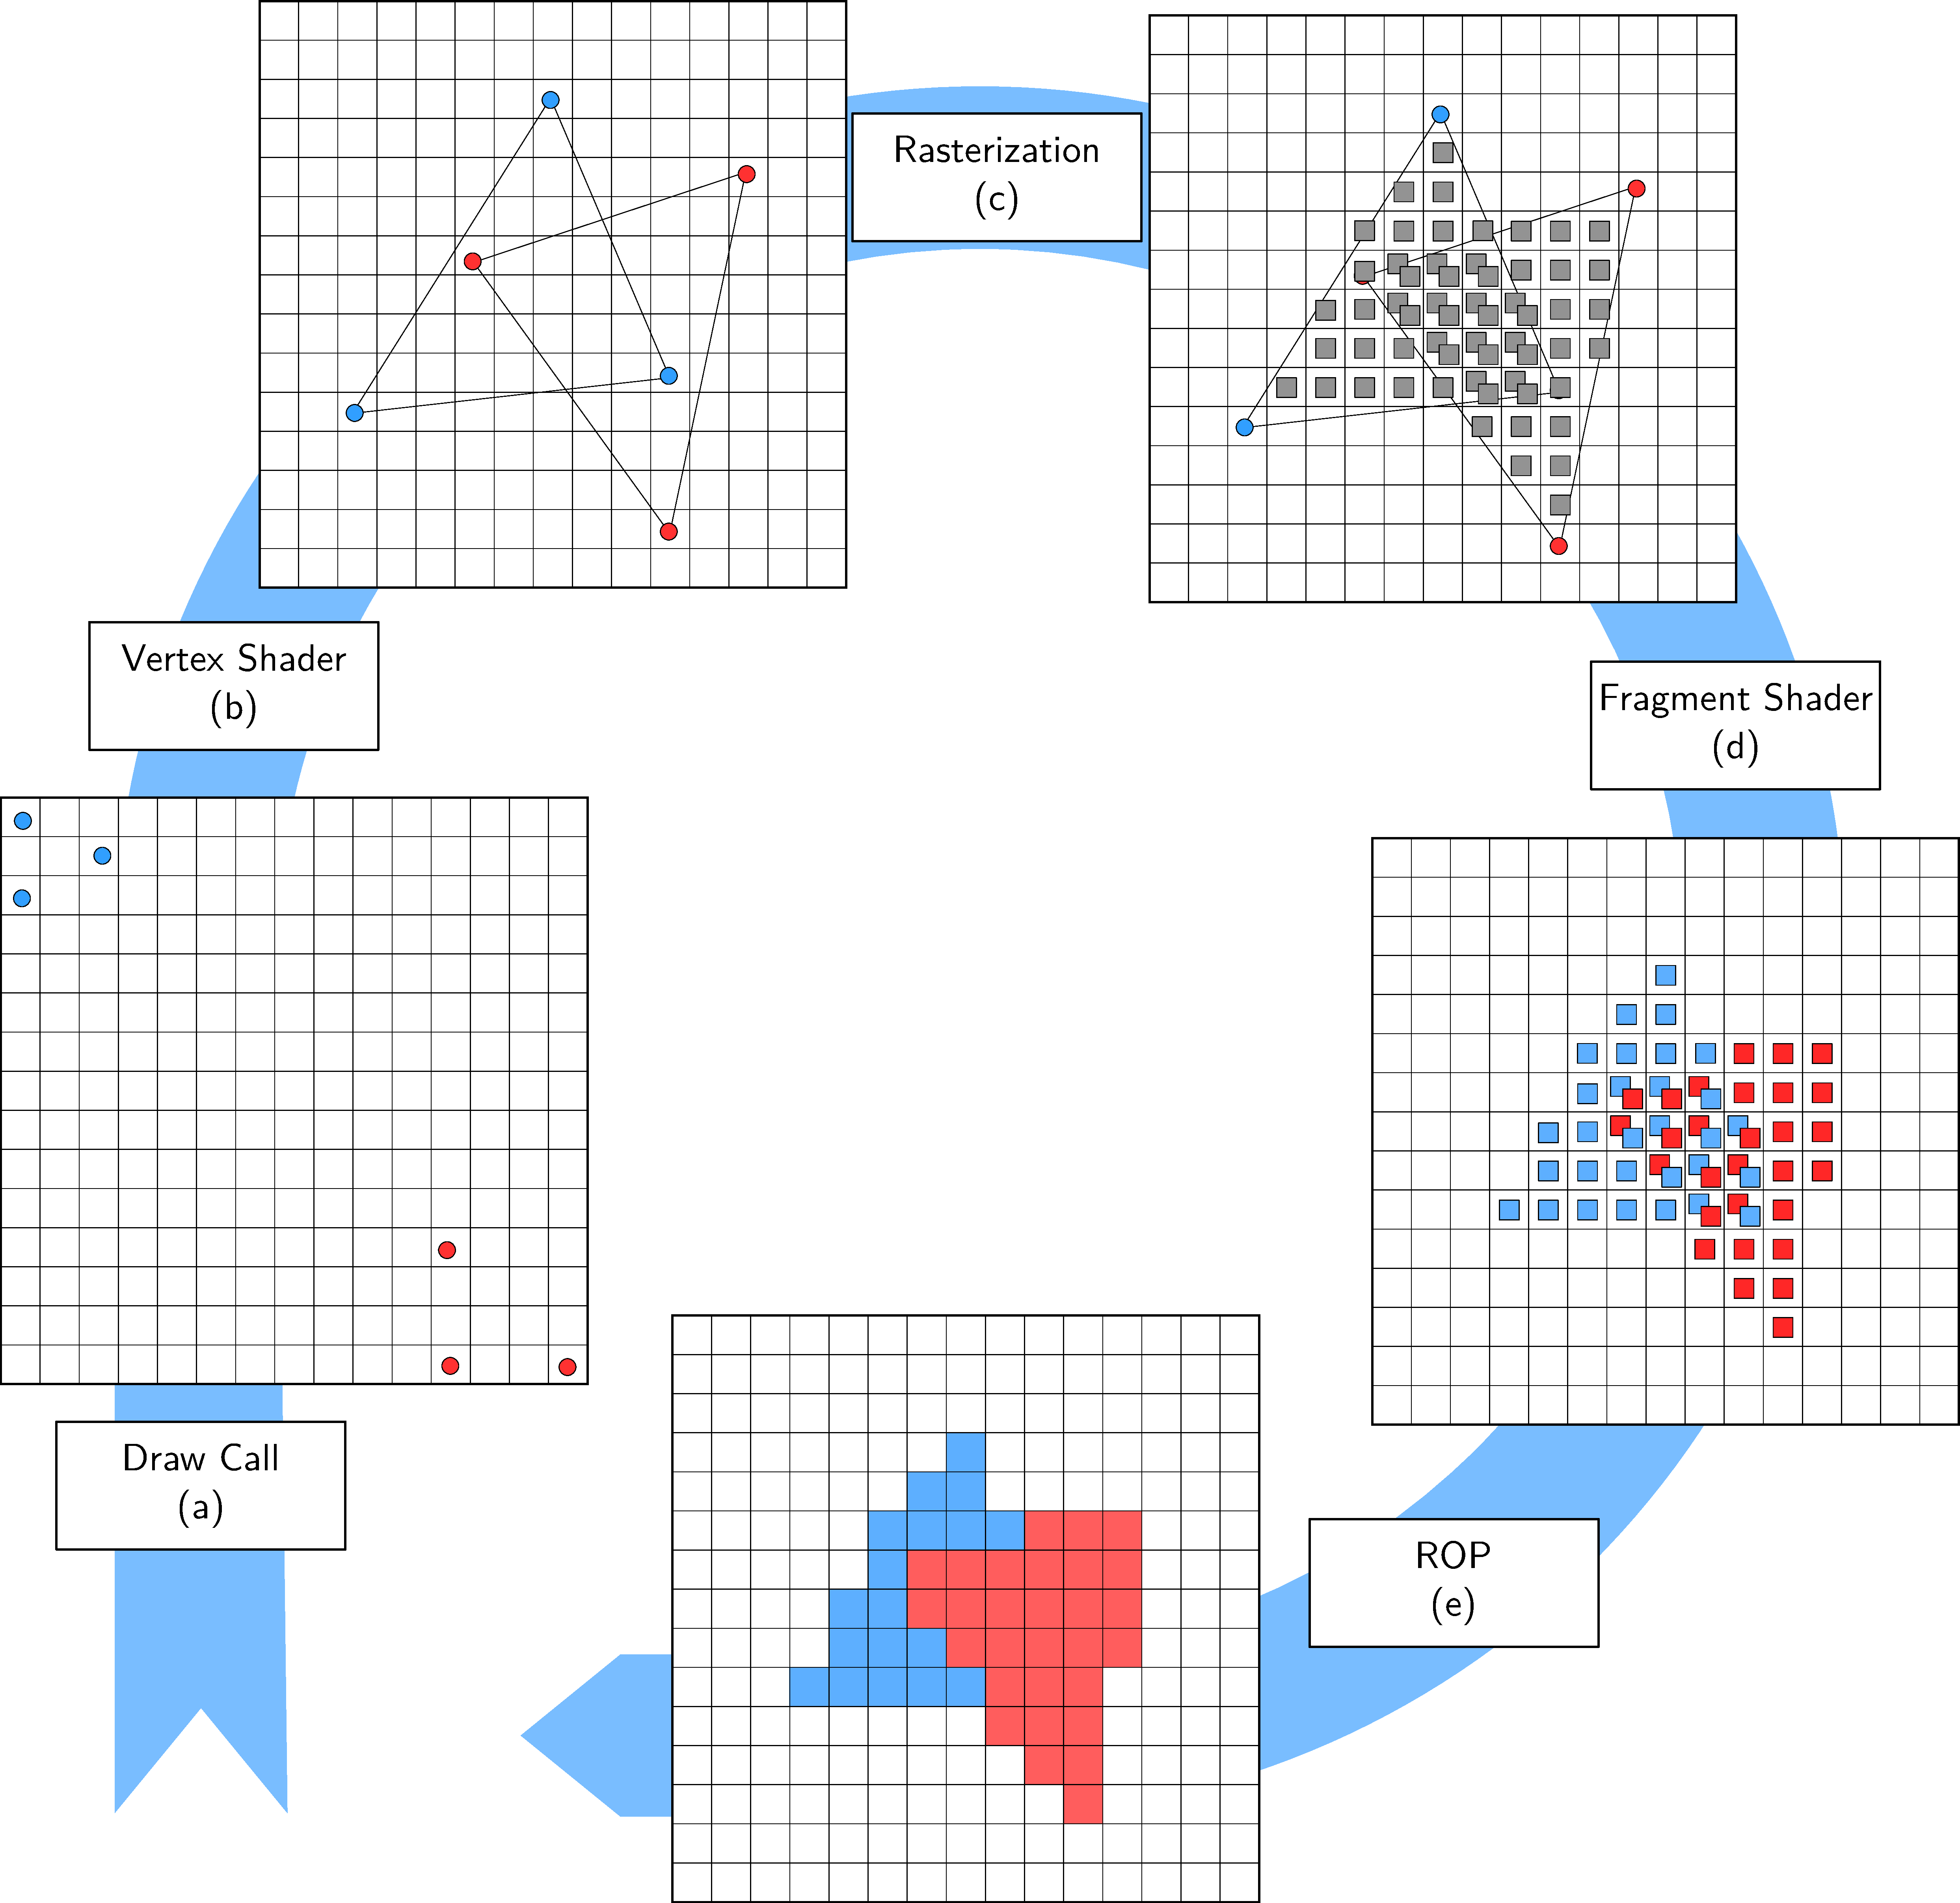
\includegraphics[width=0.85\textwidth]{figures/rasterization_pipeline.pdf} 
\caption{The rasterization pipeline. Following the arrow: bottom left, vertices in local coordinates are fetched from memory; top left, vertices are disposed by the vertex shader, then the triangle is assembled; top right, fragments (gray) are generated; bottom right, fragments are shaded; bottom, fragments are combined by a depth test to form the final image. } 
\label{fig:rasterpipeline}
\end{figure}

The first of the two techniques is rasterization. In this technique, some rendering primitives, triangles, are scanned one by one and then drawn on the screen. One example of algorithms used to transform triangles into pixel-size elements (or fragments) is scanline rendering~\cite{Wylie1967}, though it depends on the GPU vendor. By its nature, rasterization is highly parallelizable, since every primitive can be drawn in parallel. On modern graphics cards, the rasterization process is performed in hardware as part of the \emph{graphics pipeline}, a highly fine tuned sequence of steps, both hardware and software, to render triangles efficiently. A simplified version of the pipeline is illustrated in Figure~\ref{fig:rasterpipeline}. The pipeline is composed of programmable parts (called \emph{shaders}) and hardware parts, that are only controllable through state flags. The core rasterization process, transforming primitives into fragments, is executed in parallel by a specified hardware unit. 

Let us describe the life of a single triangle through the pipeline. Once the CPU issues the command to draw some triangles, a \emph{draw call} (Figure~\ref{fig:rasterpipeline}, a), the pipeline starts on the GPU. For each of the three vertices composing a triangle, we independently execute a programmable part, called the \emph{vertex shader}, that allows operation such as model and perspective transformation (Figure~\ref{fig:rasterpipeline}, b). Once the vertices have been processed, the primitive is assembled and then processed by the hardware rasterizer, generating a certain number of fragments  (Figure~\ref{fig:rasterpipeline}, c). For each fragment, we execute another programmable shader, the \emph{fragment shader}. This stage needs to output the final color of the fragment, so light interaction is usually added at this stage (Figure~\ref{fig:rasterpipeline}, d). Multiple attributes can be passed in between vertex and fragment shader, which will be interpolated using the triangle's barycentric coordinates. This allows interpolation of attributes, such as normal and texture coordinates, across the triangle, leading to a more accurate appearance. 

Once the fragments are generated, they need to be stored on the image plane. Note that multiple fragments can land on the same pixel, and that the order of landing of the fragments is not defined, since the full pipeline is entirely asynchronous. So, modern GPUs use another hardware unit, the Render OutPut unit (ROP, Figure~\ref{fig:rasterpipeline}, e) to determine how to store the fragments in the final image. This unit usually can perform depth test (via a Z-buffer) or blend the fragments, allowing us to obtain a consistent result across invocations.

This is only a simplified view of the full graphics pipeline, that, allows tessellation (domain and hull shaders), geometry manipulation (geometry shaders) or writing back into a vertex stream (transform feedback). There are also shaders that are completely detached from the graphics pipeline (compute shaders), allowing to perform tasks in parallel on the GPU that are not directly related to a graphics task. 

Rasterization is extensively used in game development and real time applications, given its high speed and predictability. However, it is not particularly well suited for propagating light across a scene, making it difficult to achieve complex optical effects, why these often require ad-hoc solutions.

\subsection{Ray tracing}
\label{sec:raytracing}
\begin{figure}
\centering
   \def\svgwidth{\textwidth}
   \input{figures/ray_tracing.pdf_tex} \\
\caption{Ray tracing four triangles in two dimensions. The thicker line corresponds to the ray (a). At each step, we consider a different bounding box (thick red border). We illustrate different cases progressively: hitting bounding box without hitting primitive (b), hitting primitive (c), hitting bounding box but not hitting primitive because triangle is behind tmax (d), updating tmax to closest primitive hit (d). The last figure (f) shows all four any hit invocation (black dots) plus the closest hit (black dot with tmax).} 
\label{fig:ray_tracing}
\end{figure}

We start this section by describing \emph{ray casting}, that can be considered the dual technique to rasterization. In rasterization, we match each triangle to its final position on the screen. In ray casting, we do the opposite: for each pixel on the screen, we find the corresponding triangles that land within that pixel. This equates to \emph{shooting} a ray through the pixel, and intersecting it though the scene geometry. Once the hit point is found, attributes can be generated and the point shaded as in a fragment shader. 

We note that, once the data structure is established, we can trace rays from any point to another in the scene. So ray tracing describes this process of querying a data structure to generate intersection points. Depending on the algorithm used, ray tracing can be used as a base of multiple rendering algorithms, such as the volume path tracing we illustrated in Section~\ref{sec:renderingscattering}. One of the first ray tracing algorithms was proposed by~\citet{Whitted1980}.

For the purpose of this thesis, we focus on GPU ray tracers. Modern GPU ray tracers build a tree data structure to efficiently lookup intersections. The most commonly used data structure is a \emph{bounding volume hierarchy}, or BVH. In a BVH, each of the primitives (usually triangles, but custom primitives such as spheres, cubes or quadrilaterals are possible) is enclosed in a bounding box. The various bounding boxes are then arranged in a tree data structure for fast lookup. Once a ray is traced, it is first inexpensively tested against the bounding boxes. For the bounding boxes that are hit, an expensive intersection test is performed to check for a hit. Depending on the shading algorithm, a callback can be issued at every encountered intersection (\emph{any hit}), or at the intersection closest to the camera (\emph{closest hit}). The process to trace a single ray in a two dimensional example is illustrated in Figure~\ref{fig:ray_tracing}. 

Many challenges need to be solved to obtain an efficient GPU ray tracer. The first challenge is recursion. In the case of an algorithm such as path tracing, a probabilistic recursive ray tracing call is performed at the closest hit. So, an efficient ray tracer needs to keep track of the state at each intersection, generically though a recursion stack (OptiX~\cite{Parker2010} is such an example, where the stack is built automatically at the instruction level). The second challenge is on how to manage the data structure if the geometry of the material changes, through deformation or animation. Simple rigid tranformations can be handled relatively inexpensively by the BVH, tough more complicated operations need to be done if  changes are performed at the single primitive level. Modern ray tracing techniques such as the TRBVH~\cite{Karras2013} can rebuild part of the BVH on the fly without excessive memory consumption. 

Given its state as a "natural" solution to light transport and its ability to model complex optical effects, ray tracing is commonly employed in the movie industry. Moreover, ray tracing scales better to scenes with a huge amount of triangles, such as in animated movies or virtual effects scenes. On the other hand, ray tracing is limited in the game developers community, due to smaller scenes and increased memory and lookup costs. Moreover, algorithms such as path tracing tend to give a noisier result, that is not acceptable in game applications. 


